% ============================================================
%  Kenya Informatics Olympiad 2026 -- First Round Paper
%  Compile with: pdflatex kio2026_round1.tex
%  Requires: rising_stars.png, cemastea_logo.png (same folder)
% ============================================================
\documentclass[a4paper,12pt]{article}
\usepackage[utf8]{inputenc}
\usepackage{geometry}
\geometry{left=2.5cm, right=2.5cm, top=2.5cm, bottom=2.5cm}
\usepackage{graphicx}
\usepackage{enumitem}
\usepackage{amsmath}
\usepackage{amssymb}
\usepackage{textcomp}
\usepackage{hyperref}
\usepackage{booktabs}
\usepackage{array}
\usepackage{tikz}
\usetikzlibrary{arrows.meta, positioning, bending}
\usepackage{multicol}

\hypersetup{colorlinks=true, linkcolor=blue, urlcolor=blue}
\setlength{\parindent}{0pt}
\setlength{\parskip}{0.7ex plus 0.2ex minus 0.2ex}

% ----------------------------------------------------------
% MCQ macros
% ----------------------------------------------------------

% Horizontal 5-choice line (for short numerical answers)
\newcommand{\hchoices}[5]{%
  \par\vspace{5pt}%
  \noindent\hspace{2em}%
  \textbf{(A)}~#1\hfill%
  \textbf{(B)}~#2\hfill%
  \textbf{(C)}~#3\hfill%
  \textbf{(D)}~#4\hfill%
  \textbf{(E)}~#5\par%
  \vspace{4pt}%
}

% Vertical 5-choice list (for longer text answers)
\newenvironment{choices}{%
  \begin{enumerate}[label=\textbf{(\Alph*)},
                    leftmargin=2.5em,
                    itemsep=2pt,
                    topsep=4pt,
                    parsep=0pt]%
}{%
  \end{enumerate}%
}

% ----------------------------------------------------------
% Title block (same structure as Round 2)
% ----------------------------------------------------------
\title{Kenya Informatics Olympiad 2026}
\author{First Round --- Selection Examination}
\date{Time allowed: 2 hours}

\makeatletter
\renewcommand{\maketitle}{%
  \begin{center}
    \begin{tabular}{ccc}
      \includegraphics[height=2.5cm]{rising_stars.png} &
      \hspace{1.5cm} &
      \includegraphics[height=2.5cm]{cemastea logo.png} \\
    \end{tabular}

    \vspace{1cm}

    {\huge\bfseries \@title\par}
    \vspace{0.3cm}
    {\large \@author\par}
    \vspace{0.2cm}
    {\normalsize \@date\par}
  \end{center}
  \vspace{0.5cm}
}
\makeatother

% ===========================================================
\begin{document}
\maketitle

% ----------------------------------------------------------
\section*{Instructions}
% ----------------------------------------------------------
\begin{itemize}
  \item Write your \textbf{full name}, \textbf{date of birth}, and \textbf{school} clearly on the answer sheet.
  \item This paper contains \textbf{20 multiple-choice questions}.
  \item For each question, select the \textbf{single best answer} and shade the corresponding
        circle --- \textbf{(A), (B), (C), (D),} or \textbf{(E)} --- on the answer sheet.
        Do not shade more than one circle per question.
  \item No calculators, phones, or electronic devices are permitted.
        Rough-work paper is provided; only the answer sheet is marked.
  \item There is \textbf{no penalty} for incorrect answers --- attempt every question.
  \item \textbf{Section A} (Questions 1--12): \textbf{1 mark} each.
        \textbf{Section B} (Questions 13--20): \textbf{2 marks} each.
        \textbf{Total: 28 marks.}
\end{itemize}

\vspace{1ex}
\hrule
\vspace{2ex}

% ===========================================================
\section*{Section A \quad\normalfont\large Basic Computational Thinking
          \hfill\normalsize(Questions 1--12, 1 Mark Each)}
% ===========================================================

\begin{enumerate}[label=\textbf{Q\arabic*.},
                  itemsep=3.5ex,
                  leftmargin=3.8em,
                  parsep=0pt]

% ----- Q1 -----
\item A delivery robot navigates a grid of streets. Intersections are at every
point $(x,y)$ where $x, y \in \{0, 1, 2, 3\}$; the bottom-left corner is
$(0,0)$ and the top-right corner is $(3,3)$. The robot starts at $(0,0)$ and
must reach $(3,3)$, moving \textbf{only East} (increasing $x$) or \textbf{only
North} (increasing $y$) at each step. The intersection at $(2,1)$ is blocked
and cannot be visited. How many valid routes are there?

\hchoices{9}{11}{14}{20}{24}

% ----- Q2 -----
\item A logic circuit has three binary inputs $A$, $B$, $C$ and one output
$Y$, built from three gates connected in sequence:

\begin{itemize}[nosep, leftmargin=2em, topsep=2pt]
  \item \textbf{AND gate}: inputs $A$ and $B$.
        Outputs $1$ \emph{only} when \emph{both} inputs are $1$; otherwise outputs $0$.
  \item \textbf{XOR gate}: inputs are the AND-gate output and $C$.
        Outputs $1$ when its two inputs \emph{differ}; outputs $0$ when they are the same.
  \item \textbf{NOT gate}: inverts the XOR-gate output to produce $Y$.
        Outputs $1$ when its input is $0$, and $0$ when its input is $1$.
\end{itemize}

What are the values of $Y$ for $(A,B,C)=(1,0,1)$ and $(A,B,C)=(1,1,1)$,
respectively?

\begin{choices}
  \item $0$ and $0$
  \item $0$ and $1$
  \item $1$ and $0$
  \item $1$ and $1$
  \item The output is undefined for these inputs
\end{choices}

% ----- Q3 -----
\item A sorted list contains exactly $1{,}000$ distinct names.
\textbf{Binary search} works as follows: compare the target name against the
\emph{middle} element of the current list; if it matches, stop; if the target
comes before the middle name, discard the second half and repeat on the first
half; otherwise discard the first half and repeat on the second half.
What is the \textbf{maximum} number of comparisons needed in the worst case?

\hchoices{9}{10}{11}{12}{7}

% ----- Q4 -----
\item A \textbf{stack} is a container where items are added and removed
from the \emph{same} end (Last In, First Out). You push the integers
$1, 2, 3, 4$ onto the stack \textbf{in that order}, freely interleaving
pushes and pops. For example: push $1$, push $2$, pop ($\to 2$), pop
($\to 1$), push $3$, pop ($\to 3$), push $4$, pop ($\to 4$) gives the
output sequence $2, 1, 3, 4$. Which of the following output sequences is
\textbf{impossible}?

\begin{choices}
  \item \texttt{1,\; 3,\; 4,\; 2}
  \item \texttt{4,\; 3,\; 2,\; 1}
  \item \texttt{3,\; 1,\; 2,\; 4}
  \item \texttt{2,\; 4,\; 3,\; 1}
  \item \texttt{3,\; 4,\; 2,\; 1}
\end{choices}

% ----- Q5 -----
\item A \textbf{binary tree} is a way of arranging items in a hierarchy.
Each item is stored in a \textbf{node} (drawn as a labelled circle). Nodes
are connected by \textbf{edges} (straight lines). One special node called the
\textbf{root} sits at the very top. Every other node has exactly one node
above it (its \textbf{parent}). Each node may have at most two nodes directly
below it: a \textbf{left child} (connected below-left) and a
\textbf{right child} (connected below-right). A \textbf{subtree} rooted at a
node means that node together with every node reachable below it.

\smallskip
Three standard ways to list all the nodes of a binary tree are:
\begin{itemize}[nosep, leftmargin=2em, topsep=3pt]
  \item \textbf{Preorder:} visit the \underline{current node first}, then list
        the left subtree, then the right subtree.
  \item \textbf{Inorder:} list the left subtree first, then visit the
        \underline{current node}, then list the right subtree.
  \item \textbf{Postorder:} list the left subtree first, then the right
        subtree, then visit the \underline{current node last}.
\end{itemize}

\medskip
\textit{Example.} The tree below has 5 nodes (labelled 1--5). Study the
diagram and verify each traversal result in the table.

\begin{center}
% ---- Tree diagram ----
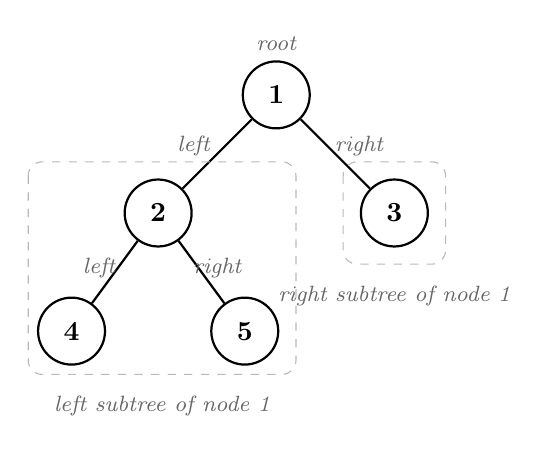
\begin{tikzpicture}[
  nd/.style={circle, draw, thick, minimum size=0.85cm, font=\bfseries},
  ed/.style={thick},
  lbl/.style={font=\footnotesize\itshape, gray!80!black}
]
  %-- Nodes
  \node[nd] (r)  at (2.8, 0)    {1};   % root
  \node[nd] (l)  at (1.3,-1.5)  {2};   % left child of 1
  \node[nd] (ri) at (4.3,-1.5)  {3};   % right child of 1
  \node[nd] (ll) at (0.2,-3.0)  {4};   % left child of 2
  \node[nd] (lr) at (2.4,-3.0)  {5};   % right child of 2

  %-- Edges
  \draw[ed] (r) -- (l);
  \draw[ed] (r) -- (ri);
  \draw[ed] (l) -- (ll);
  \draw[ed] (l) -- (lr);

  %-- Root label
  \node[lbl] at (2.8, 0.65) {root};

  %-- Left / Right edge labels (mid-edge, small italic)
  \node[lbl] at (1.75, -0.65)  {left};
  \node[lbl] at (3.85, -0.65)  {right};
  \node[lbl] at (0.55, -2.20)  {left};
  \node[lbl] at (2.05, -2.20)  {right};

  %-- Dashed box: left subtree of 1
  \draw[gray!55, dashed, rounded corners=5pt]
    (-0.35,-0.85) rectangle (3.05,-3.55);
  \node[lbl] at (1.35,-3.95) {left subtree of node 1};

  %-- Dashed box: right subtree of 1
  \draw[gray!55, dashed, rounded corners=5pt]
    (3.65,-0.85) rectangle (4.95,-2.15);
  \node[lbl] at (4.30,-2.55) {right subtree of node 1};
\end{tikzpicture}

\bigskip
% ---- Traversal table ----
\renewcommand{\arraystretch}{1.3}
\begin{tabular}{@{}lll@{}}
  \toprule
  Traversal & Rule (in words) & Result on example tree \\
  \midrule
  \textbf{Preorder}  & node, then left, then right &
    \texttt{1,\;2,\;4,\;5,\;3} \\
  \textbf{Inorder}   & left, then node, then right &
    \texttt{4,\;2,\;5,\;1,\;3} \\
  \textbf{Postorder} & left, then right, then node &
    \texttt{4,\;5,\;2,\;3,\;1} \\
  \bottomrule
\end{tabular}
\renewcommand{\arraystretch}{1}
\end{center}

\medskip
A \emph{different} binary tree has \textbf{preorder} listing
\texttt{A, B, D, E, C, F} and \textbf{inorder} listing
\texttt{D, B, E, A, F, C}. What is its \textbf{postorder} listing?

\begin{choices}
  \item \texttt{D, E, B, F, C, A}
  \item \texttt{D, B, E, F, C, A}
  \item \texttt{D, E, B, C, F, A}
  \item \texttt{E, D, B, F, C, A}
  \item \texttt{E, D, B, C, F, A}
\end{choices}

% ----- Q6 -----
\item A \textbf{graph} is a set of \textbf{vertices} (represented as labelled
dots) joined by \textbf{edges} (lines between pairs of dots). The
\textbf{degree} of a vertex is the number of edges attached to it.
An \textbf{Eulerian path} is a route through the graph that uses every edge
\emph{exactly once} --- like drawing a figure without lifting your pen or
retracing any line.

\medskip
The diagrams below show the \emph{same} four-vertex graph. The left diagram
labels each vertex with its degree. The right diagram traces one valid Eulerian
path in numbered steps ($1\to2\to3\to4\to5$), starting at~P and ending at~R.

\smallskip
\begin{center}
% Left panel: graph with degree annotations
\begin{minipage}[b]{0.44\linewidth}
\centering
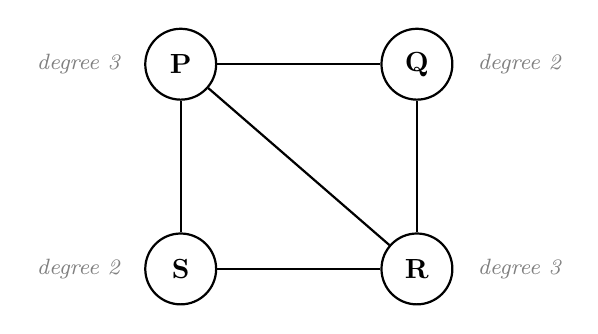
\begin{tikzpicture}[
  vx/.style={circle, draw, thick, minimum size=0.9cm, font=\bfseries},
  ed/.style={thick}
]
  \node[vx] (P) at (0,2.6)   {P};
  \node[vx] (Q) at (3,2.6)   {Q};
  \node[vx] (R) at (3,0)     {R};
  \node[vx] (S) at (0,0)     {S};

  \draw[ed] (P) -- (Q);
  \draw[ed] (Q) -- (R);
  \draw[ed] (R) -- (S);
  \draw[ed] (S) -- (P);
  \draw[ed] (P) -- (R);   % diagonal edge

  % Degree labels (outside the node)
  \node[font=\footnotesize\itshape, gray] at (-1.3,2.6) {degree~3};
  \node[font=\footnotesize\itshape, gray] at ( 4.3,2.6) {degree~2};
  \node[font=\footnotesize\itshape, gray] at ( 4.3,0)   {degree~3};
  \node[font=\footnotesize\itshape, gray] at (-1.3,0)   {degree~2};
\end{tikzpicture}
\par\smallskip
{\small\itshape P and R have \textbf{odd} degree (3).\\
Q and S have \textbf{even} degree (2).\\
Exactly 2 odd-degree vertices $\Rightarrow$\\Eulerian path exists.}
\end{minipage}%
\hfill
% Right panel: Eulerian path traced step by step
\begin{minipage}[b]{0.44\linewidth}
\centering
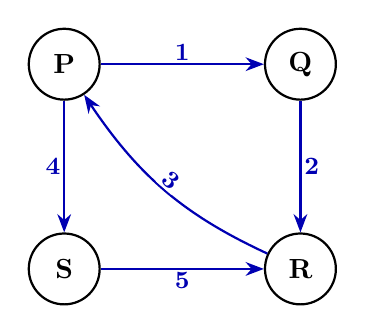
\begin{tikzpicture}[
  ->, >=Stealth,
  vx/.style={circle, draw, thick, minimum size=0.9cm, font=\bfseries},
  ep/.style={thick, blue!70!black},
  st/.style={font=\small\bfseries, fill=white, inner sep=1pt}
]
  \node[vx] (P) at (0,2.6)   {P};
  \node[vx] (Q) at (3,2.6)   {Q};
  \node[vx] (R) at (3,0)     {R};
  \node[vx] (S) at (0,0)     {S};

  \draw[ep] (P) -- node[st, above] {1} (Q);             % step 1: P→Q
  \draw[ep] (Q) -- node[st, right] {2} (R);             % step 2: Q→R
  \draw[ep] (R) to[bend left=16]
            node[st, above, sloped] {3} (P);            % step 3: R→P
  \draw[ep] (P) -- node[st, left]  {4} (S);             % step 4: P→S
  \draw[ep] (S) -- node[st, below, sloped] {5} (R);     % step 5: S→R
\end{tikzpicture}
\par\smallskip
{\small\itshape Eulerian path: P$\to$Q$\to$R$\to$P$\to$S$\to$R.\\
Every edge is used \textbf{exactly once}.}
\end{minipage}
\end{center}

\medskip
\textbf{Theorem:} A \emph{connected} graph has an Eulerian path if and only if
the number of vertices with odd degree is exactly $\mathbf{0}$
(the path forms a closed loop) or exactly $\mathbf{2}$
(the path starts at one odd-degree vertex and ends at the other).

\medskip
Which of the following graphs does \textbf{not} have an Eulerian path?

\begin{choices}
  \item Vertices $\{1,2,3,4,5\}$;\quad
        edges $(1,2),(2,3),(3,4),(4,5),(5,1)$.
  \item Vertices $\{1,2,3,4\}$;\quad
        edges $(1,2),(1,3),(1,4),(2,3),(2,4),(3,4)$.
  \item Vertices $\{1,2,3,4,5\}$;\quad
        edges $(1,2),(2,3),(3,4),(4,1),(1,5),(5,3)$.
  \item Vertices $\{1,2,3,4\}$;\quad
        edges $(1,2),(2,3),(3,4),(4,1),(1,3)$.
  \item Vertices $\{1,2,3,4,5\}$;\quad
        edges $(1,2),(2,3),(3,4),(4,5)$.
\end{choices}

% ----- Q7 -----
\item At a busy matatu terminus in Nairobi, each matatu occupies a loading bay
from its arrival until its departure; no two matatus may share a bay at the
same time. Five matatus have the following schedules:

\medskip
\begin{center}
\begin{tabular}{lcc}
  \toprule
  Matatu & Arrival (min) & Departure (min) \\
  \midrule
  1 & 10  & 100 \\
  2 & 50  & 120 \\
  3 & 90  & 150 \\
  4 & 110 & 200 \\
  5 & 140 & 180 \\
  \bottomrule
\end{tabular}
\end{center}
\medskip

What is the \textbf{minimum} number of loading bays required?

\hchoices{2}{3}{4}{5}{6}

% ----- Q8 -----
\item Katende's local computer network has 5 computers (numbered 1 to 5)
with the following \textbf{bidirectional} connections:
Computer~1 connects to Computers 2, 3, and 4;
Computer~2 connects to Computer~3;
Computer~4 connects to Computer~5.
Wesonga at Computer~1 wants to send a message to Mutua at Computer~5.
What is the minimum number of computers on any valid route from 1 to 5
\emph{(counting both endpoints)}?

\hchoices{2}{3}{4}{5}{6}

% ----- Q9 -----
\item What is the maximum number of bishops that can be placed on a standard
$8{\times}8$ chessboard so that no two bishops \textbf{threaten} each other?
A bishop threatens all squares on both of its diagonals.

\hchoices{8}{12}{14}{16}{18}

% ----- Q10 -----
\item What is the maximum number of knights that can be placed on a standard
$8{\times}8$ chessboard so that no two knights \textbf{threaten} each other?
A knight moves in an L-shape: two squares in one direction then one square
perpendicular (or vice versa).

\hchoices{16}{32}{64}{28}{40}

% ----- Q11 -----
\item A country has coins of three sizes: \textbf{1 shilling},
\textbf{3 shillings}, and \textbf{4 shillings}. You have an \textbf{unlimited
supply} of each size. The \textbf{greedy algorithm} for making change for an
amount $V$ shillings works as follows:

\begin{quote}\itshape
Repeat until the remaining amount equals zero: pick the coin with the
\textbf{largest value} that does not exceed the remaining amount, and subtract
that coin's value from the remaining amount.
\end{quote}

For example, making $V = 7$ shillings by the greedy algorithm:
\[
  7\;\xrightarrow{\;-4\;}\;3\;\xrightarrow{\;-3\;}\;0
  \qquad\text{(one 4-shilling coin + one 3-shilling coin = \textbf{2 coins}).}
\]

The greedy algorithm is not always optimal --- sometimes a different
selection of coins makes the same total using \textbf{fewer coins}.

What is the \textbf{smallest} amount $V$ (in shillings) for which the greedy
algorithm uses \textbf{strictly more coins} than the minimum possible number
of coins that can make exactly $V$ shillings?

\hchoices{5}{6}{7}{8}{9}

% ----- Q12 -----
\item You want to distribute 9 identical balls into 9 distinguishable bins,
with any number of balls (including zero) allowed in each bin.
How many distinct distributions are there?

\hchoices{$24{,}310$}{$48{,}620$}{$19{,}600$}{$11{,}440$}{$15{,}625$}

\end{enumerate}

\vspace{2ex}
\hrule
\vspace{2ex}

% ===========================================================
\section*{Section B \quad\normalfont\large Advanced Computational Thinking
          \hfill\normalsize(Questions 13--20, 2 Marks Each)}
% ===========================================================

\begin{enumerate}[label=\textbf{Q\arabic*.},
                  itemsep=3.5ex,
                  leftmargin=3.8em,
                  parsep=0pt,
                  start=13]

% ----- Q13 -----
\item A hiker in the Aberdare Ranges is given the following triangular grid of
numbers. Starting at the single top number, the hiker moves downward, at each
step choosing \textbf{one} of the two numbers immediately below the current
position. The goal is to maximise the \textbf{sum} of all numbers on the path
from top to bottom (4 numbers total). What is the maximum possible path sum?

\[
\begin{array}{*{7}{c@{\hspace{5pt}}}}
      &   &   & 5 &   &   &   \\[2pt]
      &   & 9 &   & 6 &   &   \\[2pt]
      & 4 &   & 3 &   & 7 &   \\[2pt]
    2 &   & 8 &   & 1 &   & 9 \\
\end{array}
\]

\hchoices{22}{24}{26}{27}{29}

% ----- Q14 -----
\item A \textbf{directed graph} is a collection of \emph{nodes} connected by
one-way arrows (\emph{directed edges}), each labelled with a numerical weight.
A \textbf{cycle} is a closed route that starts and ends at the same node
without visiting any other node more than once; its \textbf{total weight} is
the sum of its edge weights.

The graph below has 4 nodes and 7 directed edges.

\begin{center}
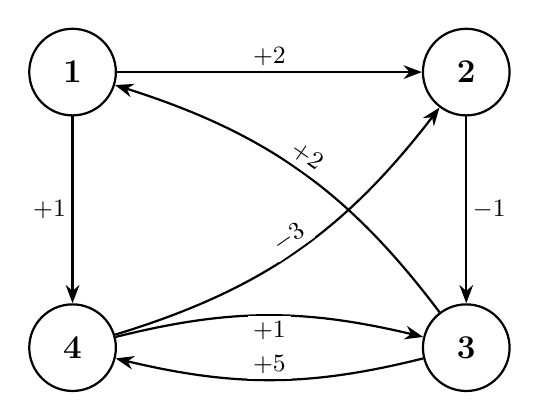
\begin{tikzpicture}[
    ->, >=Stealth, thick,
    node/.style={circle, draw, thick, minimum size=1.1cm,
                 font=\bfseries\large, fill=white},
    lbl/.style={font=\small, fill=white, inner sep=2pt}
]
  \node[node] (1) at (0,3.5) {1};
  \node[node] (2) at (5,3.5) {2};
  \node[node] (3) at (5,0)   {3};
  \node[node] (4) at (0,0)   {4};

  % Edges
  \draw (1) to node[lbl, above] {$+2$} (2);
  \draw (2) to node[lbl, right] {$-1$} (3);
  \draw (3) to[bend right=18] node[lbl, above, sloped] {$+2$} (1);
  \draw (1) to node[lbl, left]  {$+1$} (4);
  \draw (4) to[bend right=18] node[lbl, above, sloped] {$-3$} (2);
  \draw[bend left=14] (4) to node[lbl, below] {$+1$} (3);
  \draw[bend left=14] (3) to node[lbl, above] {$+5$} (4);
\end{tikzpicture}
\end{center}

Which of the following is a cycle with a \textbf{negative} total weight?

\begin{choices}
  \item Node $1 \to 2 \to 3 \to 1$
  \item Node $2 \to 3 \to 4 \to 2$
  \item Node $1 \to 4 \to 2 \to 3 \to 1$
  \item Node $1 \to 4 \to 3 \to 1$
  \item No cycle in this graph has a negative total weight
\end{choices}

% ----- Q15 -----
\item Alice and Bob each hold a \textbf{positive integer} number of sweets
and each has a \textbf{positive integer} age. They make the following
observations:

\begin{itemize}[nosep, leftmargin=2em, topsep=2pt]
  \item Alice says: \textit{``If we each add our sweets to our age, my total
        is \textbf{double} yours. If we each multiply our sweets by our age,
        my product is \textbf{four times} yours.''}
  \item Bob replies: \textit{``If you gave me 5 of your sweets, then both our
        sums \emph{and} our products (sweets $\times$ age) would be
        \textbf{equal}.''}
\end{itemize}

What is the \textbf{product of Alice's age and Bob's age}?

\hchoices{30}{40}{50}{60}{75}

% ----- Q16 -----
\item Alice and Bob play a game with a heap of \textbf{30 stones}.
Players alternate turns; on each turn the current player removes exactly
\textbf{1, 3, or 4} stones from the heap. The player who takes the
\textbf{last stone wins}.

Both players play \textbf{optimally}: each always makes the move that
guarantees their own win if a winning strategy exists; otherwise, the move
that makes things hardest for the opponent.

Alice goes first. Who wins, and what first move should they make (if applicable)?

\begin{choices}
  \item Alice wins by removing 1 stone.
  \item Alice wins by removing 3 stones.
  \item Alice wins by removing 4 stones.
  \item Bob wins; no first move by Alice can guarantee her a win.
  \item The game is a draw under optimal play.
\end{choices}

% ----- Q17 -----
\item Ten glasses stand in a row. Glass~$i$ has a capacity of exactly
$i$~litres (for $i=1,2,\ldots,10$). The glasses always contain a total of
exactly 10 litres, each holding a whole number of litres.

In one \textbf{move}, choose a source glass and a destination glass, then
pour from the source until either the source is empty or the destination is
full. No water is spilled. The \textbf{goal} is to reach the state where
every glass contains exactly 1 litre.

\medskip
\begin{center}
\begin{tabular}{lcccccccccc}
  \toprule
   & \multicolumn{10}{c}{Litres in glass $i$} \\
  \cmidrule(l){2-11}
  Configuration & 1 & 2 & 3 & 4 & 5 & 6 & 7 & 8 & 9 & 10 \\
  \midrule
  A & 0 & 2 & 1 & 1 & 1 & 1 & 1 & 1 & 1 & 1 \\
  B & 0 & 0 & 0 & 0 & 5 & 1 & 1 & 1 & 1 & 1 \\
  C & 0 & 0 & 0 & 0 & 0 & 0 & 0 & 0 & 0 & 10 \\
  \bottomrule
\end{tabular}
\end{center}
\medskip

Let $M_A$, $M_B$, $M_C$ be the minimum number of moves to reach the goal from
configurations A, B, C respectively. What is $M_A + M_B + M_C$?

\hchoices{10}{12}{14}{15}{18}

% ----- Q18 -----
\item What is the greatest number of knights that can be placed on a
$5{\times}5$ chessboard so that \textbf{every} placed knight threatens
exactly \textbf{2} other placed knights? Knights that are placed but threaten
fewer or more than 2 others are not allowed.
(\emph{A knight moves in an L-shape: two squares in one direction and one
square perpendicular.})

\hchoices{12}{14}{16}{18}{20}

% ----- Q19 -----
\item For each of the five point sets below, connect all the points with
straight-line edges to form a \textbf{simple polygon}: a single closed loop
using every point exactly once as a vertex, where no two edges cross and edges
only meet at their shared endpoints. Let $P_A, P_B, P_C, P_D, P_E$ be the
number of distinct simple polygons that can be formed from sets A, B, C, D, E
respectively. No three points in any set are collinear.

\bigskip
\begin{center}
% Top row: Sets A, B, C
\begin{minipage}[b]{0.28\linewidth}\centering
  \begin{tikzpicture}[scale=0.37]
    \foreach \x/\y in {0/0, 4/0, 6/3, 3/6, -1/4}
      \filldraw[black] (\x,\y) circle (4.5pt);
  \end{tikzpicture}
  \par\smallskip{\small\textbf{Set A} (5 points)}
\end{minipage}
\hfill
\begin{minipage}[b]{0.22\linewidth}\centering
  \begin{tikzpicture}[scale=0.37]
    \foreach \x/\y in {0/0, 5/0, 1/4, 2/1}
      \filldraw[black] (\x,\y) circle (4.5pt);
    % pad vertically to match height of A
    \vphantom{\rule{0pt}{2.2cm}}
  \end{tikzpicture}
  \par\smallskip{\small\textbf{Set B} (4 points)}
\end{minipage}
\hfill
\begin{minipage}[b]{0.28\linewidth}\centering
  \begin{tikzpicture}[scale=0.37]
    \foreach \x/\y in {0/0, 5/0, 6/4, 2/6, -1/3, 2/2}
      \filldraw[black] (\x,\y) circle (4.5pt);
  \end{tikzpicture}
  \par\smallskip{\small\textbf{Set C} (6 points)}
\end{minipage}

\bigskip

% Bottom row: Sets D and E
\begin{minipage}[b]{0.38\linewidth}\centering
  \begin{tikzpicture}[scale=0.33]
    \foreach \x/\y in {0/0, 6/0, 7/4, 4/7, 0/6, -2/3, 2/2}
      \filldraw[black] (\x,\y) circle (5pt);
  \end{tikzpicture}
  \par\smallskip{\small\textbf{Set D} (7 points)}
\end{minipage}
\hspace{3em}
\begin{minipage}[b]{0.38\linewidth}\centering
  \begin{tikzpicture}[scale=0.33]
    \foreach \x/\y in {0/0, 6/0, 7/5, 3/8, -2/5, 2/2, 4/3}
      \filldraw[black] (\x,\y) circle (5pt);
  \end{tikzpicture}
  \par\smallskip{\small\textbf{Set E} (7 points)}
\end{minipage}
\end{center}
\bigskip

What is $P_A + P_B + P_C + P_D + P_E$?

\hchoices{28}{31}{34}{37}{40}

% ----- Q20 -----
\item Exactly five of the ten integers $\{1, 2, \ldots, 10\}$ are
\textbf{``bad''}. You do not know which five. You may ask
\textbf{queries} of the form: \textit{``Does the set $Q$ contain at least
one bad integer?''}, receiving a Yes or No answer each time. What is the
\textbf{minimum} number of queries that guarantees you can always determine
the exact set of bad integers, no matter which five integers are bad?

\hchoices{8}{9}{10}{12}{14}

\end{enumerate}

\vspace{2ex}
\hrule
\vspace{1.5ex}
\begin{center}
  \Large\bfseries --- End of Paper. Good Luck! ---
\end{center}

\end{document}
